\documentclass[10pt,a4paper]{article}
\usepackage{geometry}
% \geometry{
% a4paper,
% total={210mm,297mm},
% left=20mm,
% right=20mm,
% top=20mm,
% bottom=20mm,
% }
\usepackage[utf8]{inputenc}
\usepackage[english,czech]{babel}
\usepackage{makeidx}
\usepackage{url}
\usepackage{tikz}
\usepackage{float}
\usepackage{pdfpages}
\usepackage{amsfonts}
\usepackage{mdwlist}
\usepackage{xcolor}
\usepackage{listings}
\usepackage[utf8]{inputenc}
\usepackage[T1]{fontenc}
\usepackage{listingsutf8}
\usepackage{cite}
\usepackage{hyperref}
\usepackage{booktabs}


\begin{document}
\title{Hledání nejkratší cesty v grafu}
\author{Jakub Javůrek \& Martin Beránek}
\maketitle
\newpage
\tableofcontents
\listoffigures
%\listoftables

\newpage

\section{Definice problému}

\subsection{Zadání}

Implementujte minimálně tyto algoritmy hledání nejkratších cest v grafu (mezi všema dvojicemi uzlů):
\begin{itemize}
    \item Dijkstra viz, nutná úprava algoritmu (najde všechny vzdálenosti z 1 bodu).
    \item Floydův-Warshallův algoritmus.
    \item Úkol: * x86 a Xeon.
\end{itemize}

\begin{itemize}
    \item Paralelizace obout metod, u Dijkstry každé vlákno provádí hledání z jiného startovního bodu.
    \item CUDA.
    \item Paralelizace jen Floydův-Warshallova algoritmu.
\end{itemize}

\section{Sekvenční řešení a implementace}

\subsection{Floyd Warshall algoritmus}

Floyd-Warshall algoritmus slouží k vytvoření nejkratších cest v grafu mezi všemi dvojicemi vrcholů grafu \cite{floydWarsh}. Vzdálenosti mezi vrcholy jsou zaneseny v matici přechodů, ty nesmějí mít záporné hodnoty.

Psedokód:

\begin{verbatim}
procedure [array] FloydWarshall(D, P)
    for k in 1 to n do
        for i in 1 to n do
            for j in 1 to n do
                if D[i][j] > D[i][k] + D[k][j] then
                    D[i][j] = D[i][k] + D[k][j]
                    P[i][j] = P[k][j]
    return P
\end{verbatim}

V poli P jsou uloženy předchůdci pro směrování v grafu. V poli D jsou uloženy vzdálenosti.

Složitost algoritmu je $O (|U|^3)$.

\subsubsection{Implementace}

Následující část obsahuje implementaci algoritmu v jazyce \texttt{C++}.

\begin{verbatim}
void floyd(int **matrix, int n)
{
    for (int i = 0; i < n; i++)
    {
        for (int j = 0; j < n; j++)
        {
            if (i == j)
                matrix[i][j] = 0;
            else if (matrix[i][j] == 0)
                matrix[i][j] = LARGE_INT;
        }
    }
    int i, j, k;
    for (k = 0; k < n; k++)
    {
        for (i = 0; i < n; i++)
        {
            for (j = 0; j < n; j++)
            {
                if (matrix[i][j] > matrix[i][k] + matrix[k][j])
                {
                    matrix[i][j] = matrix[i][k] + matrix[k][j];
                }
            }
        }
    }
\end{verbatim}

\subsection{Dijkstrův algoritmus}

Dijkstrův algoritmus slouží pro nalezení nejkratších cest v grafu pro jeden vrchol grafu \cite{dijskraAlg}. Algoritmus pracuje s maticí přechodu, která neobsahuje záporné hrany.

Psedokód:

\begin{verbatim}
procedure [array], [array] Dijkstra(Graph, source, D):
    create vertex set Q
      for v in Graph:
         D[v] = INFINITY
          prev[v] = UNDEFINED
          add v to Q

      D[source] = 0 
      
      while Q is not empty:
          u = vertex in Q with min D[u]
          remove u from Q 
          
          for neighbor v in u:
              alt = D[u] + length(u, v)
              if alt < D[v]:
                  dist[v] = alt 
                  prev[v] = u 
      return D, P
\end{verbatim}

\subsubsection{Implementace}

Následující část obsahuje implementaci algoritmu v jazyce \texttt{C++}.

\begin{verbatim}
int * dijsktra(int ** edgeMatrix, int vertexCnt, int s){
    int * p = new int[vertexCnt];
    int * d = new int[vertexCnt];
    set <int> * N = new set<int>;
    for (int i = 0; i < vertexCnt; i++){
        d[i] = LARGE_INT; // infinity
        p[i] = -1; // uknown
        N->insert(i);
    }
    d[s] = 0;
    int next = s;
    while (!N->empty()){
        int u = next;
        N->erase(u);
        next = *N->begin();

        set<int>::iterator it;
        for (it = N->begin(); it != N->end(); ++it)
        {
            if (edgeMatrix[u][*it] > 0)
            {
                int alt = d[u] + edgeMatrix[u][*it];
				if(alt < d[*it]){
					d[*it] = alt;
				}
                if (alt < d[*it]){
                    p[*it] = u;
                }
            }
            if (d[next] > d[*it])
                next = *it;
        }
    }
    return d;
}
\end{verbatim}

Jelikož je v zadáno, že výsledkem musí být obsahovat vzdálenost všech vrcholy, je algoritmus volán postupně se všemi vrcholy grafu.

\section{Instance dat}

Pro oba algoritmy byla sestavená matice s velikostí $4000x4000$ s celkovou velikostí 31\,MB. Matice byla generována pomocí předepsané aplikace \texttt{generator}. Následně byla upravena do jiné formy pro změnění vzdáleností mezi body. Z vygenerovaných vzdáleností 1 se stali náhodná čísla v řádu desítek.

Pro náhled je uveden začátek matice:

\begin{verbatim}
4000
0 0 0 0 0 0 0 0 0 0 0 0 0 0  ...
0 0 0 0 8 0 0 0 0 0 0 0 0 0  ...
0 0 0 0 0 0 0 0 0 0 0 0 0 0  ...
0 0 4 0 0 0 0 0 0 0 0 0 0 0  ...
. . . . . . . . . . . . . . 
. . . . . . . . . . . . . . 
. . . . . . . . . . . . . . 
\end{verbatim}

\section{OpenMP}

\subsection{Floyd Warshall algoritmus}

Algoritmus byl upraven o direktivy pro překladač, který zapínají \texttt{OpenMP}. Vektorizaci bylo možné použít po úpravě podmínky v \texttt{for} cyklu. Byla nahrazena funkcí \texttt{min}.

\begin{verbatim}
void floyd(int **matrix, int n, int threadCnt)
{
    for (int i = 0; i < n; i++)
    {
        for (int j = 0; j < n; j++)
        {
            if (i == j)
                matrix[i][j] = 0;
            else if (matrix[i][j] == 0)
                matrix[i][j] = LARGE_INT;
        }
    }
    if (threadCnt > 0)
        omp_set_num_threads(threadCnt); // nastavení počtu vláken

    int i, j, k;
    for (k = 0; k < n; k++)
    {
        #pragma omp parallel for private(i,j) // direktiva pro OpenMP
        for (i = 0; i < n; i++)
        {
            for (j = 0; j < n; j++)
            {
                // upraveno pro vektorizaci
                matrix[i][j] = min(matrix[i][j], matrix[i][k] + matrix[k][j]);
            }
        }
    }

}
\end{verbatim}

Překladač cyklus nevektorizoval s odůvodněním:

\begin{verbatim}
floyd.cpp:36: note: not vectorized: not suitable for gather load _33 = *_32;
floyd.cpp:36: note: bad data references.
\end{verbatim}

K vektorizaci nedošlo kvůli nekonzistentní alokované paměti.

\subsection{Dijkstrův algoritmus}

Jedinou změnou pro Dijkstrův algoritmus bylo přidání \texttt{OpenMP} direktiv. Větší změny nebyly možné kvůli velkým datovým závislostem ve \texttt{for} cyklech. Ačkoliv bylo přidání jedno volání funkce \texttt{min}, zrychlení nebylo žádné, protože data, nad kterými je funkce vykována, závisí na zbytku těla cyklu.

Dalším problémem je použití složité datové struktury pro hledání minima v grafu. Práce s ní algoritmus samozřejmě ještě víc zpomaluje.

\begin{verbatim}
    if (threadCnt > 0)
        omp_set_num_threads(threadCnt); // nastavení počtu vláken

    #pragma omp parallel for private(j) // direktiva pro OpenMP
    for(j = 0; j < stc; j++){
        d[j] = dijsktra(matrix, stc, j);
    }


int * dijsktra(int ** edgeMatrix, int vertexCnt, int s){
    int * p = new int[vertexCnt];
    int * d = new int[vertexCnt];
    set <int> * N = new set<int>;
    for (int i = 0; i < vertexCnt; i++){
        d[i] = LARGE_INT; // infinity
        p[i] = -1; // uknown
        N->insert(i);
    }
    for (int i = 0; i < vertexCnt; i++){
        N->insert(i);
    }   
    d[s] = 0;
    int next = s;
    while (!N->empty()){
        int u = next;
        N->erase(u);
        next = *N->begin();

        set<int>::iterator it;
        for (it = N->begin(); it != N->end(); ++it)
        {
            if (edgeMatrix[u][*it] > 0)
            {
                int alt = d[u] + edgeMatrix[u][*it];
                d[*it] = min(alt, d[*it]);
                if (alt < d[*it]){
                    p[*it] = u;
                }
            }
            if (d[next] > d[*it])
                next = *it;
        }
    }
    return d;
}
\end{verbatim}

Překladač nevektorizoval cyklus hlavního výpočtu s odůvodněním:
\begin{verbatim}
dijks.cpp:32: note: not vectorized: control flow in loop.
\end{verbatim}

K vektorizaci nedošlo kvůli řídícím strukturám v cyklu. 

Naopak se povedl vektorizovat výpočet na začátku funkce nastavující \texttt{LARGE\_INT} a \texttt{-1}. Překladač vypsal zprávu:

\begin{verbatim}
Vectorizing loop at dijks.cpp:20
dijks.cpp:20: note: create runtime check for data references LARGE_INT and *_27
dijks.cpp:20: note: create runtime check for data references LARGE_INT and *_30
dijks.cpp:20: note: create runtime check for data references *_27 and *_30
dijks.cpp:20: note: created 3 versioning for alias checks.
dijks.cpp:20: note: === vect_do_peeling_for_loop_bound ===
Setting upper bound of nb iterations for epilogue loop to 2
dijks.cpp:20: note: LOOP VECTORIZED.
dijks.cpp:15: note: vectorized 1 loops in function.
dijks.cpp:20: note: Completely unroll loop 2 times
\end{verbatim}

\subsection{Naměřená data}

První měření proběhlo na \texttt{Intel(R) Xeon(R) CPU E5-2620 v2 @ 2.10GHz}. První měření proběhlo na Intel(R) Xeon(R) CPU E5-2620 v2 @ 2.10GHz. Počet vláken provádějících výpočet byl zvyšován v následující řadě: 1, 2, \dots , 24. Měření probíhalo pomocí skriptu v noci s kontrolou, zdali na clusteru nejsou další uživatelé. Měření proběhlo ve tři hodiny ráno z noci z neděle na pondělí.

Doby výpočtu je v následující tabulce (\ref{tab:xnfl}):
\begin{table}[H]
  \centering
	\caption{Čas výpočtu Floyd Warshall algoritmu}
	\begin{tabular}{| l | r |}
\hline
Počet vláken & Rychlost ve vteřinách \\ \hline
1 & 155.992 \\ \hline
2 & 79.9949 \\ \hline
3 & 53.5526 \\ \hline
4 & 40.3126 \\ \hline
5 & 33.2484 \\ \hline
6 & 28.4757 \\ \hline
7 & 29.1981 \\ \hline
8 & 27.3738 \\ \hline
9 & 29.5177 \\ \hline
10 & 30.8656 \\ \hline
11 & 29.0657 \\ \hline
12 & 29.0995 \\ \hline
13 & 32.1369 \\ \hline
14 & 31.6199 \\ \hline
15 & 29.4036 \\ \hline
16 & 30.7675 \\ \hline
17 & 28.1378 \\ \hline
18 & 29.7564 \\ \hline
19 & 27.2729 \\ \hline
20 & 29.3864 \\ \hline
21 & 27.3018 \\ \hline
22 & 29.6423 \\ \hline
23 & 27.0364 \\ \hline
24 & 29.5721 \\ \hline
	\end{tabular}
  \label{tab:xnfl}
\end{table}


\begin{figure}[H]
  \centering
    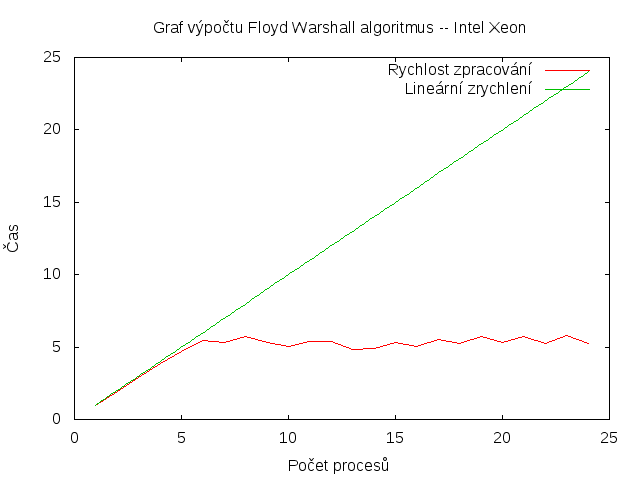
\includegraphics[width=0.8\textwidth]{graf_floyd_intel.png}
  \caption{Graf zrychlení výpočtu Floyd}
  \label{fig:floyd}
\end{figure}

Zrychlení Floyd Warshallova algoritmu pro velké počty vláken přestává držet lineární zrychlení.


\begin{table}[H]
  \centering
	\caption{Čas výpočtu Dijkstra algoritmu}
	\begin{tabular}{| l | r |}
\hline
Počet vláken & Rychlost ve vteřinách \\ \hline
1 & 360.883 \\ \hline
2 & 170.996 \\ \hline
3 & 120.683 \\ \hline
4 & 90.68 \\ \hline
5 & 72.2292 \\ \hline
6 & 57.0565 \\ \hline
7 & 51.7025 \\ \hline
8 & 43.2244 \\ \hline
9 & 40.1845 \\ \hline
10 & 34.5069 \\ \hline
11 & 31.6283 \\ \hline
12 & 29.3998 \\ \hline
13 & 31.0053 \\ \hline
14 & 32.7462 \\ \hline
15 & 30.2443 \\ \hline
16 & 31.1353 \\ \hline
17 & 28.8648 \\ \hline
18 & 28.312 \\ \hline
19 & 28.4545 \\ \hline
20 & 27.6419 \\ \hline
21 & 26.5522 \\ \hline
22 & 25.8142 \\ \hline
23 & 25.2867 \\ \hline
24 & 24.6004 \\ \hline
	\end{tabular}
  \label{tab:djfl}
\end{table}

\begin{figure}[H]
  \centering
    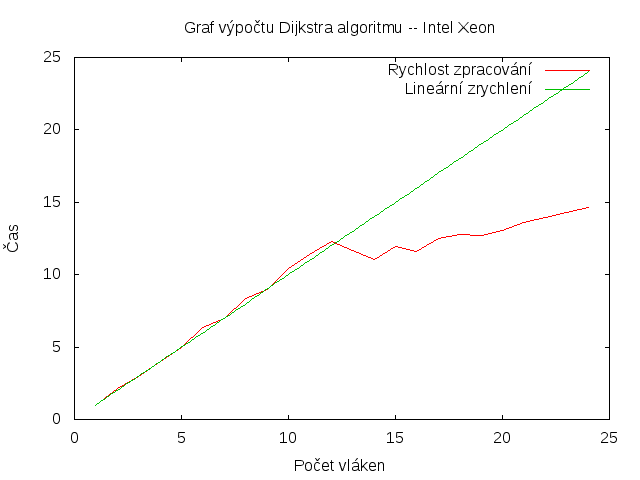
\includegraphics[width=0.8\textwidth]{graf_dijkstra_intel.png}
  \caption{Graf zrychlení výpočtu Dijkstra}
  \label{fig:dijk}
\end{figure}

Zrychlení algoritmu se drží lineárního zrychlení. Důvodem také může být, že celý výpočet je v jedné instanci o řád pomalejší, než v případu Floyd Warshalla. Ve velkých počtech instancí se však doba zpracování přestává lišit.

Druhé měření proběhlo na Intel(R) Xeon(R) Phi(TM). Měření proběhlo pomocí skriptu v době, kdy na clusteru nikdo jiný nebyl. Měření tedy mohlo proběhnout v řadě 1, 2, \dots , 244 vláken.

V následující tabulce jsou uvedeny pouze referenční hodnoty (\ref{tab:djph}):

\begin{table}[H]
  \centering
	\caption{Čas výpočtu Floyd Warshall algoritmu}
	\begin{tabular}{| l | r |}
\hline
Počet vláken & Rychlost ve vteřinách \\ \hline
1 & 1337.32 \\ \hline
10 & 142.572 \\ \hline
20 & 68.1147 \\ \hline
30 & 48.1608 \\ \hline
40 & 35.6807 \\ \hline
50 & 31.3623 \\ \hline
60 & 25.2053 \\ \hline
70 & 24.6364 \\ \hline
80 & 21.6174 \\ \hline
90 & 19.6177 \\ \hline
100 & 19.7071 \\ \hline
110 & 17.9346 \\ \hline
120 & 16.7724 \\ \hline
130 & 17.9536 \\ \hline
140 & 18.7667 \\ \hline
150 & 16.861 \\ \hline
160 & 15.9678 \\ \hline
170 & 14.9669 \\ \hline
180 & 14.3501 \\ \hline
190 & 19.8682 \\ \hline
200 & 15.6912 \\ \hline
210 & 17.896 \\ \hline
220 & 17.7623 \\ \hline
230 & 17.6404 \\ \hline
240 & 16.5851 \\ \hline
	\end{tabular}
  \label{tab:djph}
\end{table}

\begin{figure}[H]
  \centering
    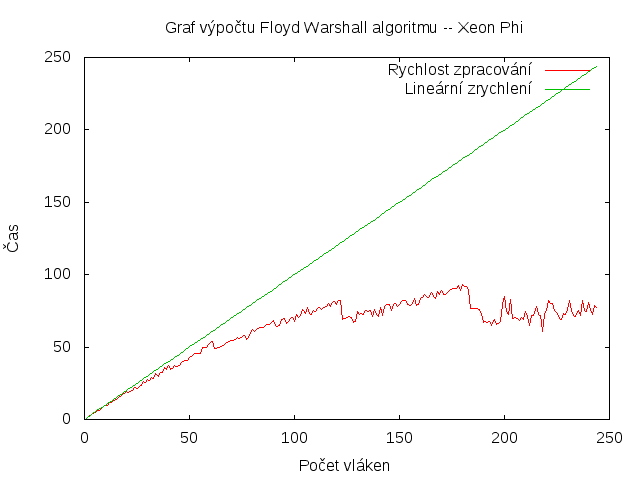
\includegraphics[width=0.8\textwidth]{graf_floyd_phi.png}
  \caption{Graf zrychlení výpočtu Floyd}
  \label{fig:floydphi}
\end{figure}

Zrychlení Floyd Warshallova algoritmu pro velké počty vláken přestává držet lineární zrychlení. Výkyvy po 61 jádrech ukazují na omezení v počtu vláken na kartu. V případě počtu vláken 62 jsou zabraná všechna jádra a jedno z nich pracuje se dvěma vlákny. Tím je celý výpočet zpomalen. Zrychlení se vylepšuje s použitím více 9 vláken na jádro. K největšímu zrychlení došlo při použití 183 vláken ($3 \cdot 61$).

\begin{table}[H]
  \centering
	\caption{Čas výpočtu Dijkstra algoritmu}
	\begin{tabular}{| l | r |}
\hline
Počet vláken & Rychlost ve vteřinách \\ \hline
1 & 2622.89 \\ \hline
10 & 253.226 \\ \hline
20 & 123.594 \\ \hline
30 & 93.7867 \\ \hline
40 & 67.3802 \\ \hline
50 & 55.222 \\ \hline
60 & 45.397 \\ \hline
70 & 49.7902 \\ \hline
80 & 42.7281 \\ \hline
90 & 41.8506 \\ \hline
100 & 35.6632 \\ \hline
110 & 34.7739 \\ \hline
120 & 30.6839 \\ \hline
130 & 42.5086 \\ \hline
140 & 39.5326 \\ \hline
150 & 37.6043 \\ \hline
160 & 36.0399 \\ \hline
170 & 34.2481 \\ \hline
180 & 32.6829 \\ \hline
190 & 40.1083 \\ \hline
200 & 38.612 \\ \hline
210 & 37.8351 \\ \hline
220 & 37.9962 \\ \hline
230 & 36.09 \\ \hline
240 & 34.1638 \\ \hline

	\end{tabular}
  \label{tab:daph}
\end{table}


\begin{figure}[H]
  \centering
    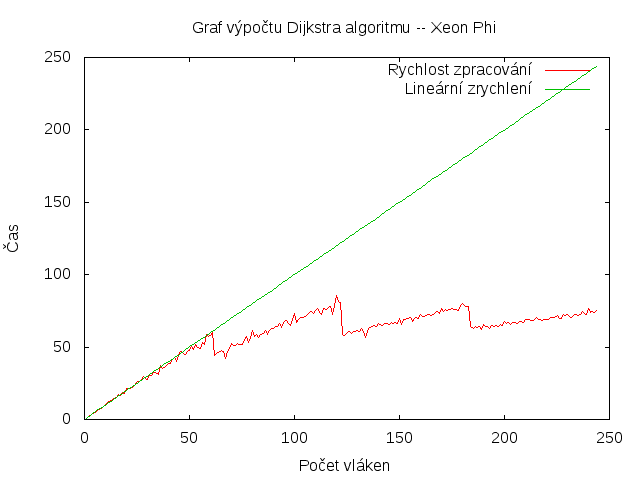
\includegraphics[width=0.8\textwidth]{graf_dijkstra_phi.png}
  \caption{Graf zrychlení výpočtu Dijkstra}
  \label{fig:dijkphi}
\end{figure}

Zrychlení Dijkstra algoritmu pro velké počty vláken přestává držet lineární zrychlení. Na grafu je vidět jev, který byl už na měření Floyd Warshall algoritmu. Největší zrychlení nastalo při 122 vláknech.

\section{CUDA}

\subsection{Floyd Warshall algoritmus}

Volání grafické karty předchází inicializace a kopírování matice do \texttt{CUDA} zařízení. Prostor vláken výpočtu je rozdělen ve dvou dimenzích pomocí \texttt{dim3} gridu.

\begin{verbatim}
void gpu_floyd(int *matrix, int n){
  int *cumatrix; 
  cudaMalloc((void **)&cumatrix, n * n * sizeof(int));
  cudaMemcpy(cumatrix, matrix,  n * n * sizeof(int), cudaMemcpyHostToDevice);
  
  dim3 dimGrid(( n + BLOCK_SIZE - 1 ) / BLOCK_SIZE, n);
  
  floyd_prepare<<<dimGrid, BLOCK_SIZE>>>(cumatrix, n);
  
  cudaThreadSynchronize();
     
  for (int k = 0; k < n; k++){
    floyd_kern<<<dimGrid, BLOCK_SIZE>>>(k, cumatrix, n);
    cudaThreadSynchronize();  
  }
  
  cudaMemcpy(matrix, cumatrix, sizeof(int)*n*n,cudaMemcpyDeviceToHost);  
  cudaFree(cumatrix);
}
\end{verbatim}

Velikost bloku je stejná jako počet použitých vláken. Jejich dělení je na obrázku (\ref{fig:grid}). Celý prostor je rozdělen tedy do dvou dimenzí rozdělených podle počtu alokovaných vláken.

\begin{figure}[H]
  \centering
    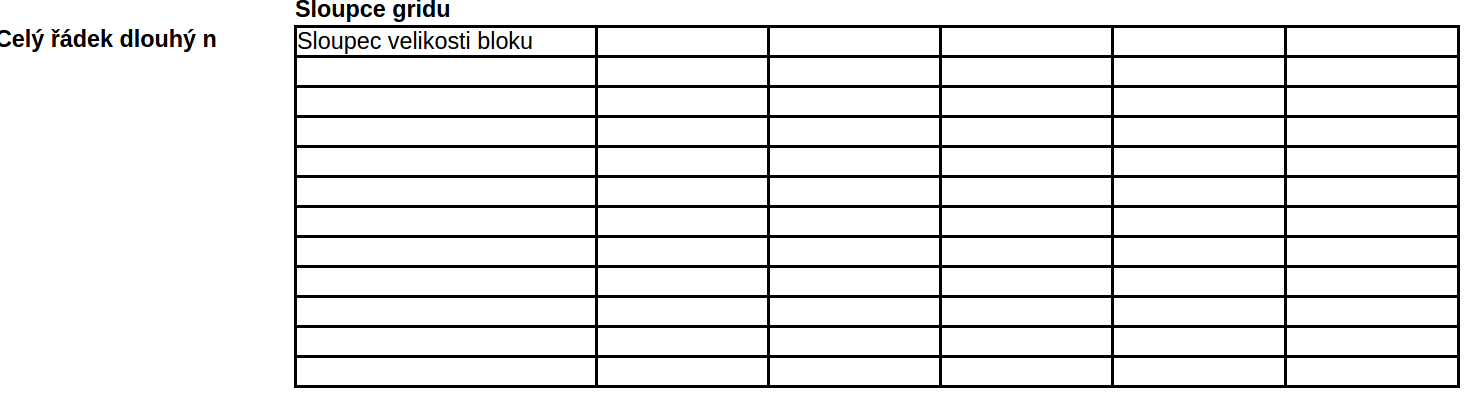
\includegraphics[width=0.8\textwidth]{grid.png}
  \caption{Rozmístění vláken v gridu}
  \label{fig:grid}
\end{figure}

Následně se zavolá funkce \texttt{floyd\_prepare}, která na grafické kartě nastaví matici pro výpočet algoritmu. Po dokončení výpočtu se zavolá samotný algoritmus.

\begin{verbatim}
__global__ void floyd_prepare(int *matrix, int n){
  int column = blockIdx.x * blockDim.x + threadIdx.x;
  int idx = n * blockIdx.y + column;
  if(column >= n )
      return;
  if ( blockIdx.y == column)
    matrix[idx] = 0;
  else if(matrix[idx] == 0)
    matrix[idx] = INT_MAX/2;
}
\end{verbatim}

Výpočet algoritmu \cite{cudaFloyd}: 

\begin{verbatim}
__global__ void floyd_kern(int k, int *matrix, int n){
  int column = blockIdx.x * blockDim.x + threadIdx.x; // pozice na radku
  if(column >= n ) // pokud přepluje, pravděpodobně jsme přejeli velikost bloku
      return;
  int idx = n * blockIdx.y + column; // přesná pozice v matici
  
  __shared__ int bmatch; // pro jedno k nejlepší hodnota v floyd
  
  if(threadIdx.x == 0)
      bmatch = matrix[n*blockIdx.y + k];
  
  __syncthreads();
  
  if(bmatch == INT_MAX/2)
     return;
  
  int tmp = matrix[k*n+column];
  
  if(tmp == INT_MAX/2) 
    return;
  
  int current = bmatch + tmp;
  if(current < matrix[idx]){
    matrix[idx] = current; // matrix[i*n+j] = min(matrix[i*n+j], matrix[i*n+k] + matrix[k*n+j]);
  }
}
\end{verbatim}

Na rozdíl od řešení pomocí cyklů každé vlákno představuje jeden samostatný kousek výpočtu. Všechna součastně běžící vlákna mezi sebou sdílí \texttt{bmatch}, který představuje \texttt{matrix[i*n+k]}. Podle umístěná v gridu se rozhodnou, zdali je nejlepší cestou současná hodnota nebo součet \texttt{tmp} a \texttt{bmatch}, které představují \texttt{matrix[i*n+k] + matrix[k*n+j]}. V případě, že je \texttt{bmatch} nebo \texttt{tmp} roven nekonečnu, pak nemohou představovat v součtu nejlepší cestu a vlákno se ukončuje.

Měření proběhne pomocí měnění velikosti proměnnné \texttt{BLOCK\_SIZE}, která představuje velikost sloupce v řádku a také počet vláken, které v buňce tabulky pracují.

\subsection{Naměřená data}

První měření probíhalo na \texttt{GTS 650 Ti}. 

\begin{table}[H]
  \centering
	\caption{Čas výpočtu Floyd Warshall algoritmu na GTS 650 Ti v milisekundách}
	\begin{tabular}{| l | r |}
\hline
Počet vláken & Rychlost ve vteřinách \\ \hline
40 & 27695.6 \\ \hline
80 & 14280.9 \\ \hline
120 & 10626.7 \\ \hline
160 & 10237 \\ \hline
200 & 11102.6 \\ \hline
240 & 10616.3 \\ \hline
280 & 10881.6 \\ \hline
320 & 10617.4 \\ \hline
360 & 11483.2 \\ \hline
400 & 12095 \\ \hline
440 & 11870.1 \\ \hline
480 & 11299.5 \\ \hline
520 & 13275.9 \\ \hline
560 & 13277.6 \\ \hline
600 & 13277.2 \\ \hline
640 & 13278.1 \\ \hline
680 & 13277.2 \\ \hline
720 & 13277.2 \\ \hline
760 & 13278.5 \\ \hline
800 & 13277.8 \\ \hline
840 & 13277.4 \\ \hline
880 & 13278.1 \\ \hline
920 & 13104.1 \\ \hline
960 & 12701 \\ \hline
1000 & 12376.3 \\ \hline
	\end{tabular}
  \label{tab:cufl}
\end{table}


\begin{figure}[H]
  \centering
    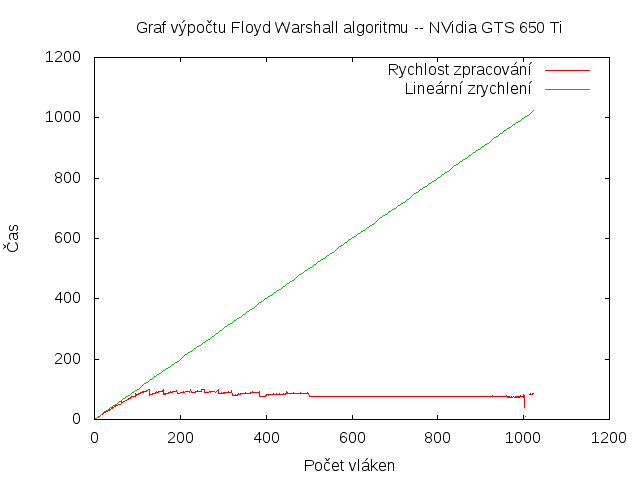
\includegraphics[width=0.8\textwidth]{graf_floyd_gts_650_Ti.png}
  \caption{Graf zrychlení výpočtu Floyd Warshall}
  \label{fig:floydcuda}
\end{figure}


Druhé měření probíhalo na \texttt{GTS 780 Ti} na školním clusteru \texttt{star.fit.cvut.cz}.

\begin{table}[H]
  \centering
	\caption{Čas výpočtu Floyd Warshall algoritmu na GTS 780 Ti v milisekundách}
	\begin{tabular}{| l | r |}
\hline
Počet vláken & Rychlost ve vteřinách \\ \hline
33 & 13517.8 \\ \hline
99 & 3383.1 \\ \hline
165 & 3184.83 \\ \hline
231 & 3024.53 \\ \hline
264 & 4341.66 \\ \hline
297 & 3113.47 \\ \hline
363 & 4447.31 \\ \hline
429 & 3211.24 \\ \hline
495 & 4469.42 \\ \hline
561 & 5044.13 \\ \hline
594 & 4665.71 \\ \hline
627 & 4701.09 \\ \hline
693 & 5699.16 \\ \hline
759 & 3928.79 \\ \hline
825 & 5163.5 \\ \hline
891 & 3555.05 \\ \hline
924 & 5157.97 \\ \hline
957 & 5192.25 \\ \hline
1023 & 13610.1 \\ \hline
	\end{tabular}
  \label{tab:cufltwo}
\end{table}


\begin{figure}[H]
  \centering
    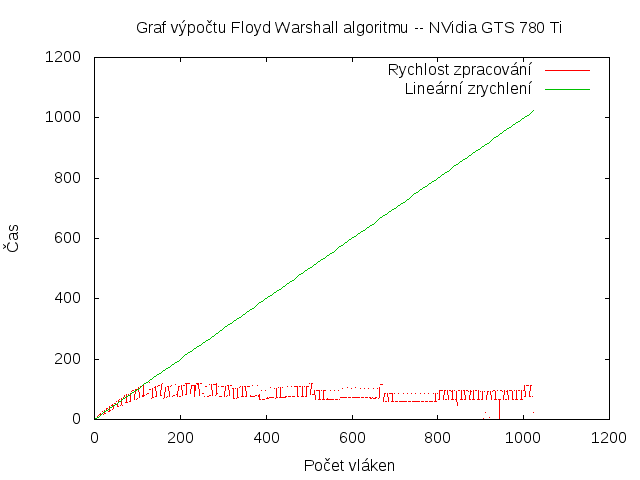
\includegraphics[width=0.8\textwidth]{graf_floyd_gts_780_Ti.png}
  \caption{Graf zrychlení výpočtu Floyd Warshall}
  \label{fig:floydcudatwo}
\end{figure}

\subsection{Dijkstrův algoritmus}

Volání grafické karty předchází inicializace a kopírování matice do \texttt{CUDA} zařízení. Prostor vláken výpočtu je rozdělen ve dvou dimenzích. Počet bloků odpovídá počtu uzlů děleným počtem vláken v bloku. Počet vláken v bloku je definován v \texttt{BLOCK\_SIZE}.

\begin{verbatim}
.
.
.
int *cumatrix; 
int *d;
cudaMalloc((void **)&cumatrix, stc * stc * sizeof(int));
cudaMemcpy(cumatrix, matrix,  stc * stc * sizeof(int), cudaMemcpyHostToDevice);
cudaMalloc((void **)&d, stc * stc * sizeof(int));

prepareArray<<<stc / BLOCK_SIZE, BLOCK_SIZE>>>(stc, d);
cudaError_t code = cudaThreadSynchronize();  
if (code != cudaSuccess)
{
  fprintf(stdout, "GPUassert: %s \n", cudaGetErrorString(code));
}

dijsktra<<<stc / BLOCK_SIZE, BLOCK_SIZE>>>(cumatrix, stc, d);
code = cudaThreadSynchronize();  
if (code != cudaSuccess)
{
  fprintf(stdout, "GPUassert: %s \n", cudaGetErrorString(code));
}
  
int *outM = new int[stc*stc];
cudaMemcpy(outM, d,  stc * stc * sizeof(int), cudaMemcpyDeviceToHost);
.
.
.
\end{verbatim}

Následně se zavolá funkce \texttt{prepareArray}, která na grafické kartě nastaví matici pro výpočet algoritmu. Po dokončení výpočtu se zavolá samotný algoritmus.

\begin{verbatim}
__global__ void prepareArray(int vertexCnt, int* d)
{
  int threads = gridDim.x * gridDim.y * gridDim.z * blockDim.x * blockDim.y * blockDim.z; //celkovy pocet vlaken
  int cycleCnt = (vertexCnt / threads > 0 ? vertexCnt / threads : 1); //velikost prace vlakna
  for (int cycle = 0; cycle < cycleCnt; cycle++)
  {
    int s = (blockIdx.x * blockDim.x + threadIdx.x) + threads * cycle;
    if(s >= vertexCnt) 
      return;

    for (int i = 0; i < vertexCnt; i++)
    {
      d[vertexCnt *i+s] = INT_MAX / 2;
    }
  }
}
\end{verbatim}

Jelikož na grafické kartě nelze použít implementaci ADT množiny std::set, vytvořili jsme pro naše účely jednoduchou vlastní implementaci:
\begin{verbatim}
class mySet
{
private:
  int size = 4000;
  bool N[4000]; //pro nase ucely staci takto omezit
  int cnt = 4000;
	
public:
  __device__ mySet(){}
	
  __device__ void init(int s)
  {
    this->cnt = s;
    for (int i = 0; i < s; i++)
    {
      N[i] = true;
    }
  }

  __device__ bool contains(int x)
  {
    return N[x];
  }

  __device__ void insert(int x)
  {
    if (N[x] == true)
      return;
    N[x] = true;
    cnt++;
  }

  __device__ void erase(int x)
  {
    if (N[x] == true)
    {
      N[x] = false;
      cnt--;
    }
  }

  __device__ bool empty()
  {
    return (cnt == 0);
  }

  __device__ int getCount()
  {
    return cnt;
  }
};
\end{verbatim}

Výpočet algoritmu:

\begin{verbatim}
__global__ void dijsktra( int* __restrict__ edgeMatrix, int vertexCnt, int* d)
{
  int threads = gridDim.x * gridDim.y * gridDim.z * blockDim.x * blockDim.y * blockDim.z;
  int cycleCnt = (vertexCnt / threads > 0 ? vertexCnt / threads : 1); //velikost prace vlakna
  for (int cycle = 0; cycle < cycleCnt; cycle++)
  {
    int s = (blockIdx.x * blockDim.x + threadIdx.x) + threads * cycle;
    if(s >= vertexCnt) 
      return;
			
    mySet N; 
		
    N.init(vertexCnt);

    d[s*vertexCnt + s] = 0;
    while (!N.empty())
    {
      int localMin = INT_MAX;

      int cnt = N.getCount();
      int u = 0;
      int j = 0;
      for (int i = 0; i < vertexCnt && j < cnt; i++)
      {
        if (!N.contains(i)) continue;
        if (localMin > d[vertexCnt *i+s])
        {
          localMin = d[vertexCnt *i+s];
          u = i;
        }
        j++;
      }
      N.erase(u);

      for (int i = 0; i < vertexCnt; i++)
      {
        if (i == u || !N.contains(i)) continue;

        if (edgeMatrix[u + i*vertexCnt] > 0)
        {
          int alt = d[vertexCnt *u+s] + edgeMatrix[u + i*vertexCnt];
          atomicMin((d + vertexCnt * i + s), alt);
        }
      }
    }
  }
}
\end{verbatim}

Idea za algoritmem je jednoduchá - vlákna si rozdělí matici grafu po sloupcích a postupně zpracovávají svůj přídel práce.

Měření proběhne pomocí měnění velikosti proměnnné \texttt{BLOCK\_SIZE}, která představuje počet vláken, které v buňce tabulky pracují.

\subsection{Naměřená data}

Zde měření probíhalo pouze na \texttt{GTS 780 Ti} na školním clusteru \texttt{star.fit.cvut.cz}.

\begin{table}[H]
  \centering
	\caption{Čas výpočtu Dijkstrova algoritmu na GTS 780 Ti v milisekundách}
	\begin{tabular}{| l | r |}
\hline
Počet vláken & Rychlost ve vteřinách \\ \hline
11 & 97627.6 \\ \hline
31 & 50964.5 \\ \hline
47 & 38982.1 \\ \hline
91 & 33748.9 \\ \hline
151 & 33750 \\ \hline
255 & 33738 \\ \hline
403 & 34409 \\ \hline
575 & 33763.7 \\ \hline
763 & 23035.4 \\ \hline
855 & 23018.2 \\ \hline
951 & 23042.7 \\ \hline
1023 & 23030.5 \\ \hline
	\end{tabular}
  \label{tab:cufltwo}
\end{table}


\begin{figure}[H]
  \centering
    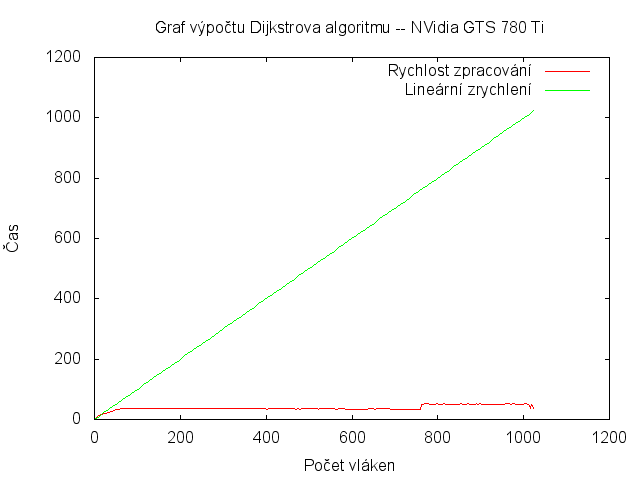
\includegraphics[width=0.8\textwidth]{graf_dikstra_gts_780_Ti.png}
  \caption{Graf zrychlení výpočtu Dijkstrova algoritmu}
  \label{fig:dijkscuda}
\end{figure}


\newpage

\section{Závěr}

Při paralelizaci na procesoru Intel Xeon dosahujeme většího zrychlení u dijkstrova algoritmu. Floyd-Warshallův zrychluje nejvíce 6x, kdežto dijkstrův až 12x - zřejmě lépe využívá virtuální vlákna. Díky tomu dosahují při vyšším počtu vláken oba algoritmy srovnatelných výsledků, přestože při sekvenčním běhu je Floyd-Warshallův přibližně dvakrát rychlejší (pro měřená vstupní data).

Při běhu na akcelerátoru Intel Xeon Phi dojde při vyšším počtu vláken k zanedbatelnému zrychlení u Floyd-Warshalla. Dijkstrův algoritmus je naopak mírně pomalejší - projevují se datové závislosti.
Na obou grafech lze vidět úpadek ve výkonu při počtech vláken v intervalech po 61. Projevuje se zde omezení počtu vláken na kartu.

Implementace Floyd-Warshallova algoritmu v CUDA zrychluje prakticky lineárně přibližně do 100 vláken. Poté se již pohybuje okolo stálé konstanty. Dijkstrův algoritmus zrychluje jen asi do 50 vláken, poté je zde ještě menší skok okolo 800. Horší škálování je dáno jednak implmentací, druhak datovými závislostmi algoritmu.

Srovnáme-li časy výpočtů dosažené na grafické kartě s těmi z klasického CPU nebo akcelerátoru Xeon Phi vidíme, že u GPU dosahujeme zdaleka nejhorších výsledků - i při nejvyšších dosažených zrychleních se nevyrovnáme sekvenčnímu řešení na CPU.

Podle výsledků všech měření se zdá, že problém hledání nejkratší cesty je (za použití našich implementaci obou algoritmů)
nejvýhodnější řešit na standardním CPU, zde Intel Xeon 2620 v2. 

\newpage

\bibliographystyle{csn690}
\bibliography{literatura}

\end{document}
